\documentclass[nooutcomes]{ximera}
%% handout
%% space
%% newpage
%% numbers
%% nooutcomes

%I added the commands here so that I would't have to keep looking them up
%\newcommand{\RR}{\mathbb R}
%\renewcommand{\d}{\,d}
%\newcommand{\dd}[2][]{\frac{d #1}{d #2}}
%\renewcommand{\l}{\ell}
%\newcommand{\ddx}{\frac{d}{dx}}
%\everymath{\displaystyle}
%\newcommand{\dfn}{\textbf}
%\newcommand{\eval}[1]{\bigg[ #1 \bigg]}

%\begin{image}
%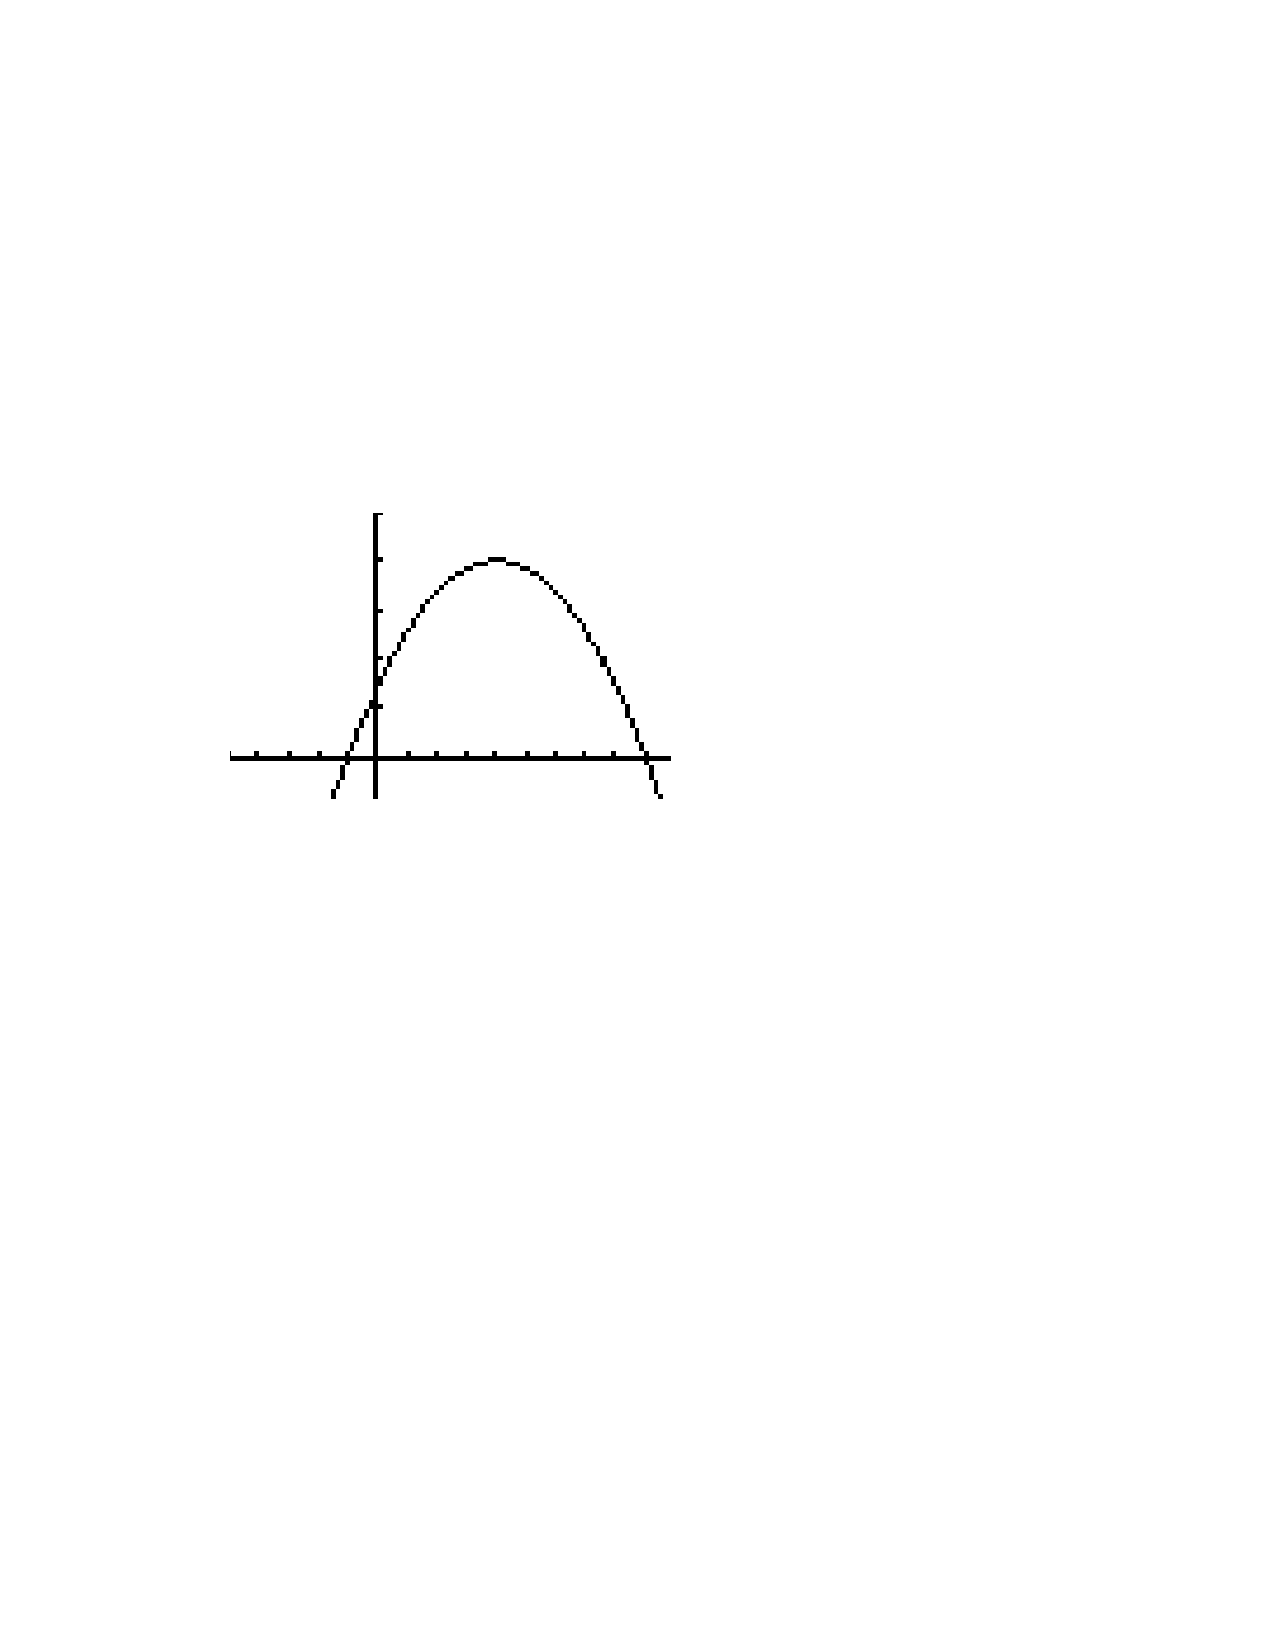
\includegraphics[trim= 170 420 250 180]{Figure1.pdf}
%\end{image}
\usepackage{fullpage}

\newcommand{\RR}{\mathbb R}
\renewcommand{\d}{\,d}
\newcommand{\dd}[2][]{\frac{d #1}{d #2}}
\renewcommand{\l}{\ell}
\newcommand{\ddx}{\frac{d}{dx}}
\newcommand{\dfn}{\textbf}
\newcommand{\eval}[1]{\bigg[ #1 \bigg]}

\usepackage{multicol}

\renewenvironment{freeResponse}{
\ifhandout\setbox0\vbox\bgroup\else
\begin{trivlist}\item[\hskip \labelsep\bfseries Solution:\hspace{2ex}]
\fi}
{\ifhandout\egroup\else
\end{trivlist}
\fi} %% we can turn off input when making a master document

\title{1.4B and 3.10: Derivatives of Inverse Trig Functions}  

\begin{document}
\begin{abstract}		\end{abstract}
\maketitle

%problem1
\begin{problem}
Explain what each of the following means:
	\begin{enumerate}
	
	%part a
	\item  $\sin^{-1}(x)$
		\begin{freeResponse}
		This denotes the inverse function to $\sin(x)$, sometimes denoted by $\arcsin(x)$.  
		\end{freeResponse}	
		
	%part b
	\item  $\left( \sin(x) \right)^{-1}$
		\begin{freeResponse}
		This means $\sin(x)$ raised to the $-1$ power, i.e. $\frac{1}{\sin(x)}$.  
		\end{freeResponse}	
		
	%part c
	\item  $\sin \left(x^{-1} \right)$
		\begin{freeResponse}
		This means $\sin \left( \frac{1}{x} \right)$.
		\end{freeResponse}	
		
	\end{enumerate}
\end{problem}

%problem2
\begin{problem}
 Without using a calculator, determine if the equation
  \[
    \cos^{-1}\bigl(\cos(7\pi/6)\bigr) = 7\pi/6
  \]
  is true or false.
  \begin{freeResponse}
    This statement is \textbf{false}: the correct equation is $\cos^{-1}\bigl(\cos(7\pi/6)\bigr) = 5\pi/6$. (Why?)

    \textbf{Spoiler Alert}: the cosine function is \emph{not} invertible since its graph fails the horizontal line test.
    \begin{image}
      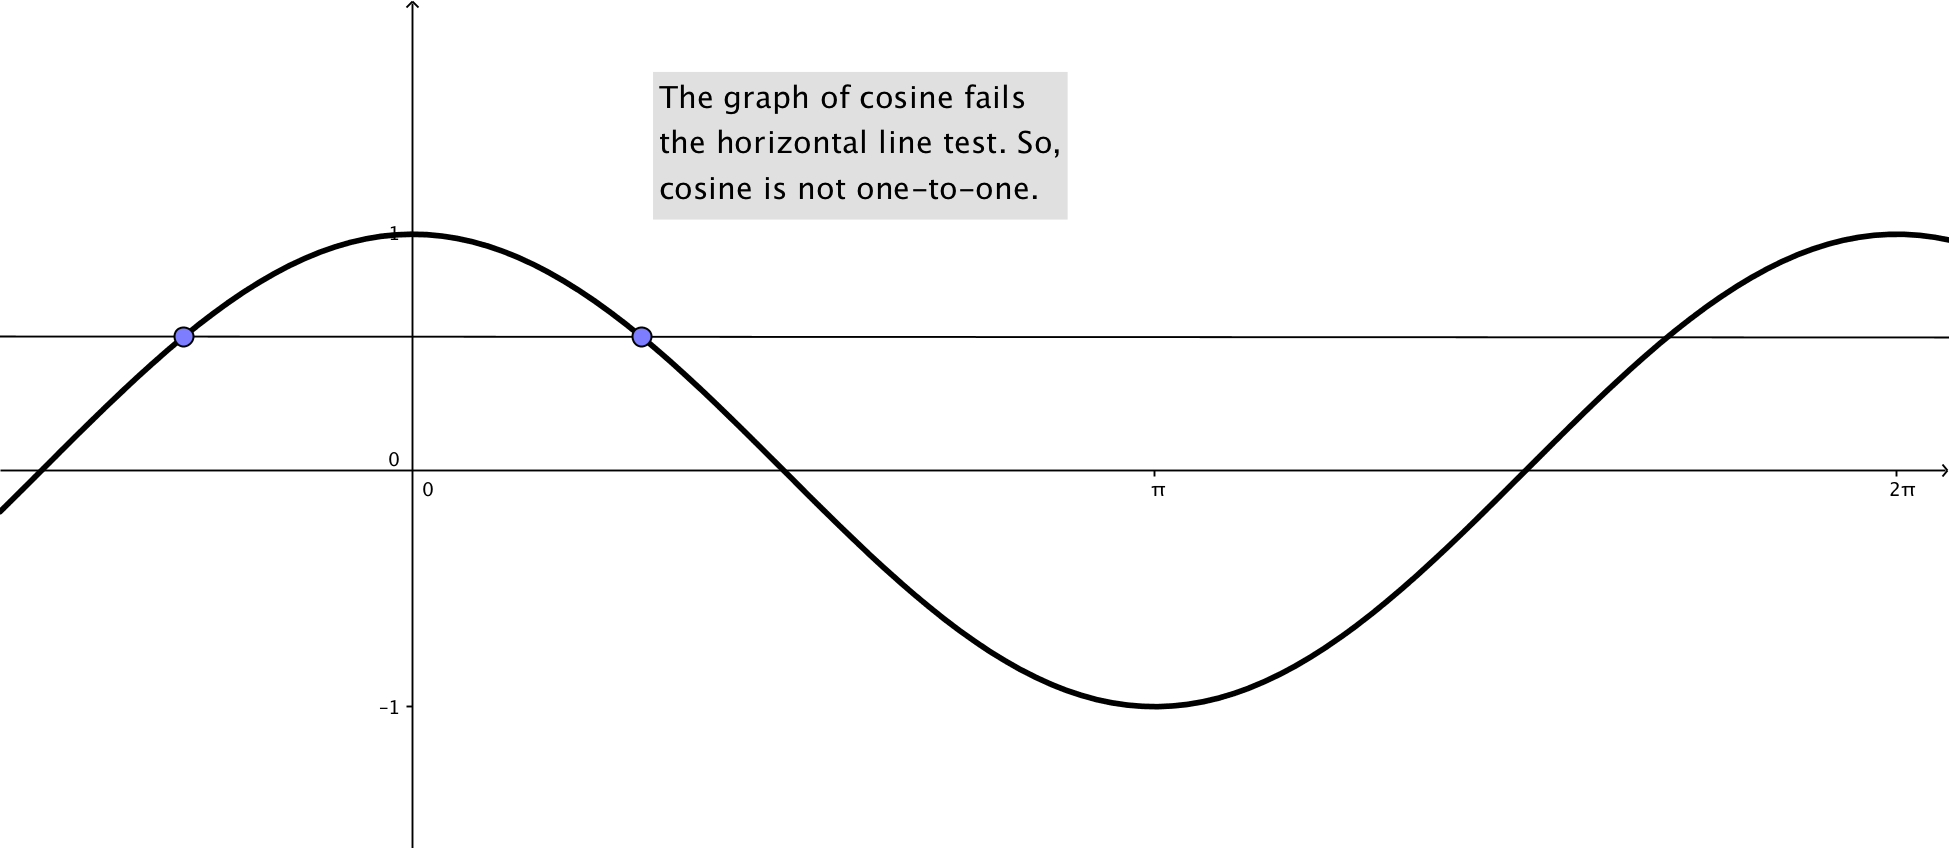
\includegraphics[scale = 0.8]{figure1.png}
    \end{image}
    To produce the inverse cosine we must first restrict the domain of cosine, to the interval $[0, \pi]$, to produce an invertible function:
    \begin{image}
      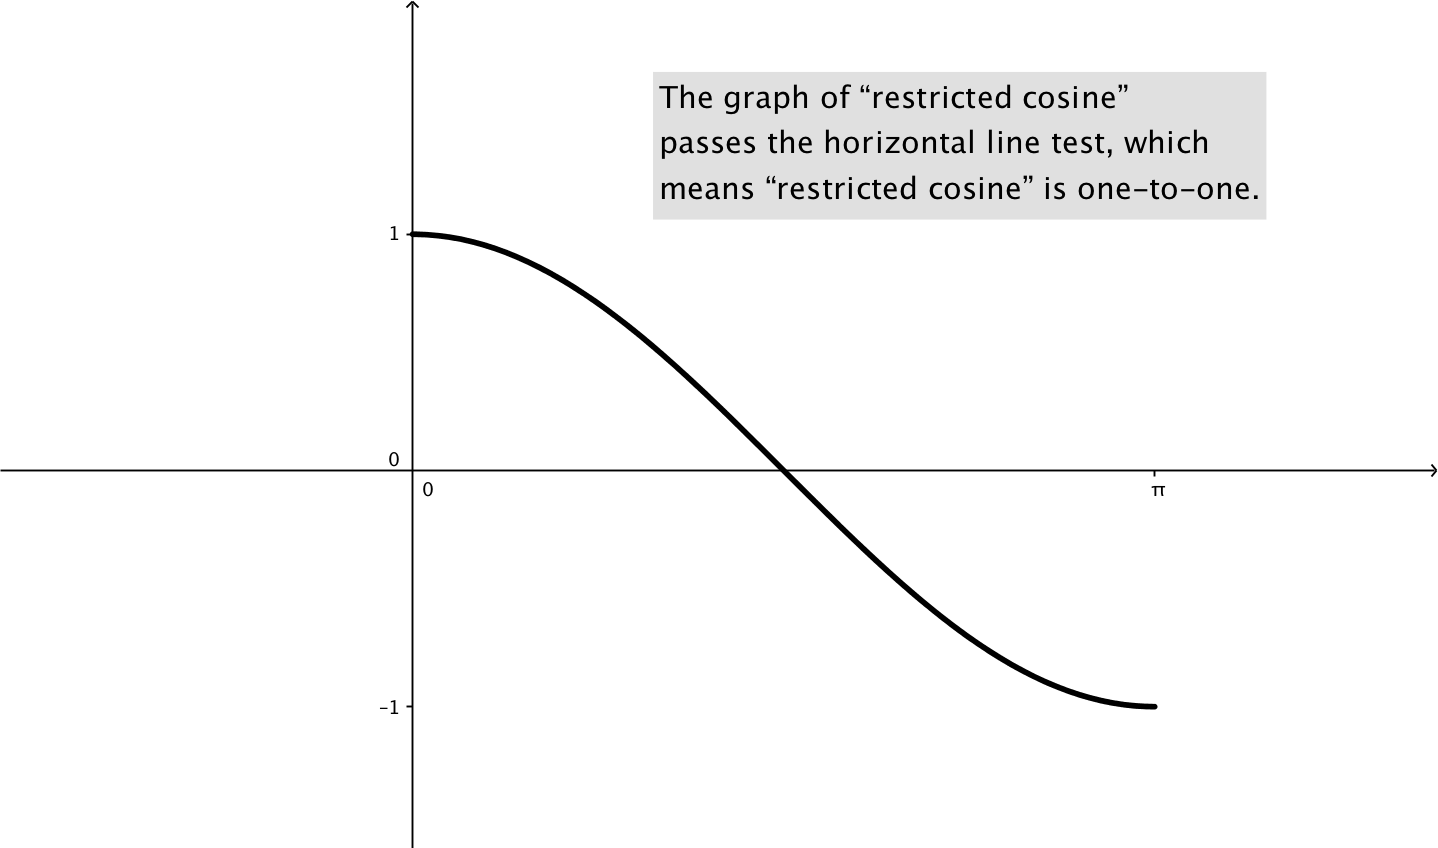
\includegraphics[scale = 0.8]{figure2.png}
    \end{image}
    So, the range of $\cos^{-1}$ is $[0, \pi]$.
    Since $7\pi/6$ is not in this range, $7\pi/6$ is \emph{never} a possible output of $\cos^{-1}$.
  \end{freeResponse}
\end{problem}

%problem3
\begin{problem}

  \textbf{True or False:}
  $\sin^{-1}(0) = \pi$.
  \begin{freeResponse}
    This statement is \textbf{false}: the correct equation is $\sin^{-1}(0) = 0$. (Why?)

    \textbf{Spoiler Alert}: the sine function is \emph{not} invertible since its graph fails the horizontal line test.
    \begin{image}
      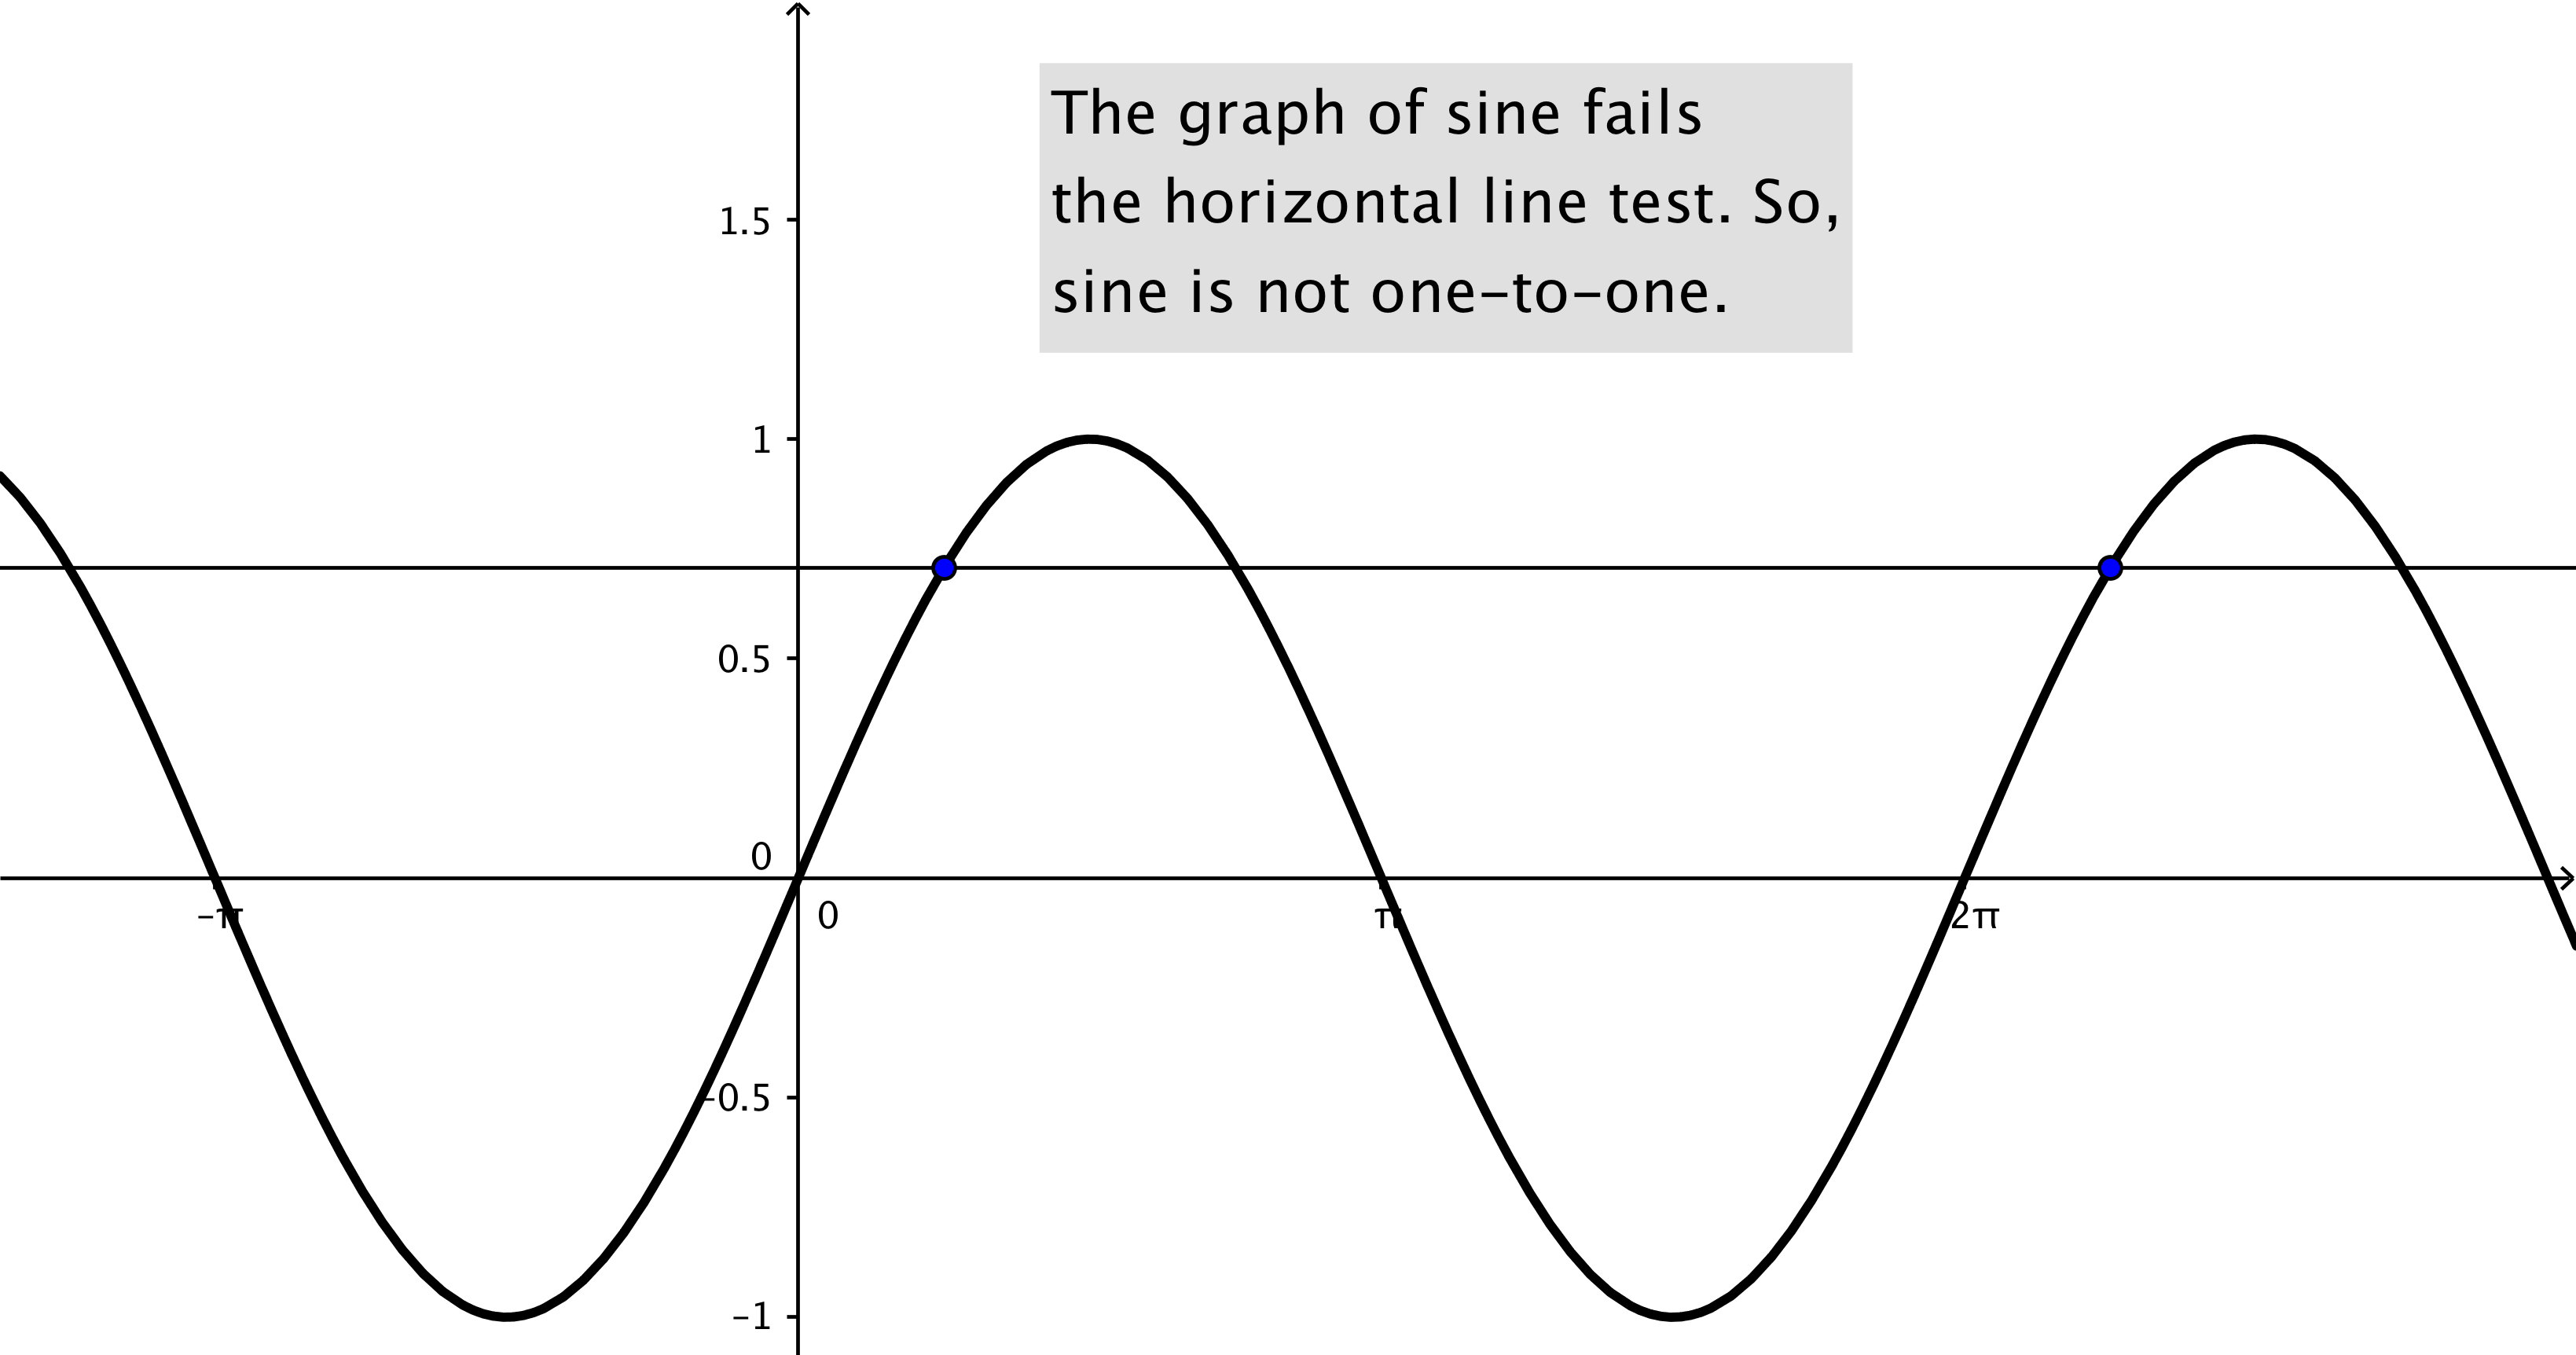
\includegraphics[scale = 0.4]{figure3.png}
    \end{image}
    To produce the inverse sine we first restrict the domain of sine, to the interval $[-\pi/2, \pi/2]$, to produce an invertible function:
    \begin{image}
      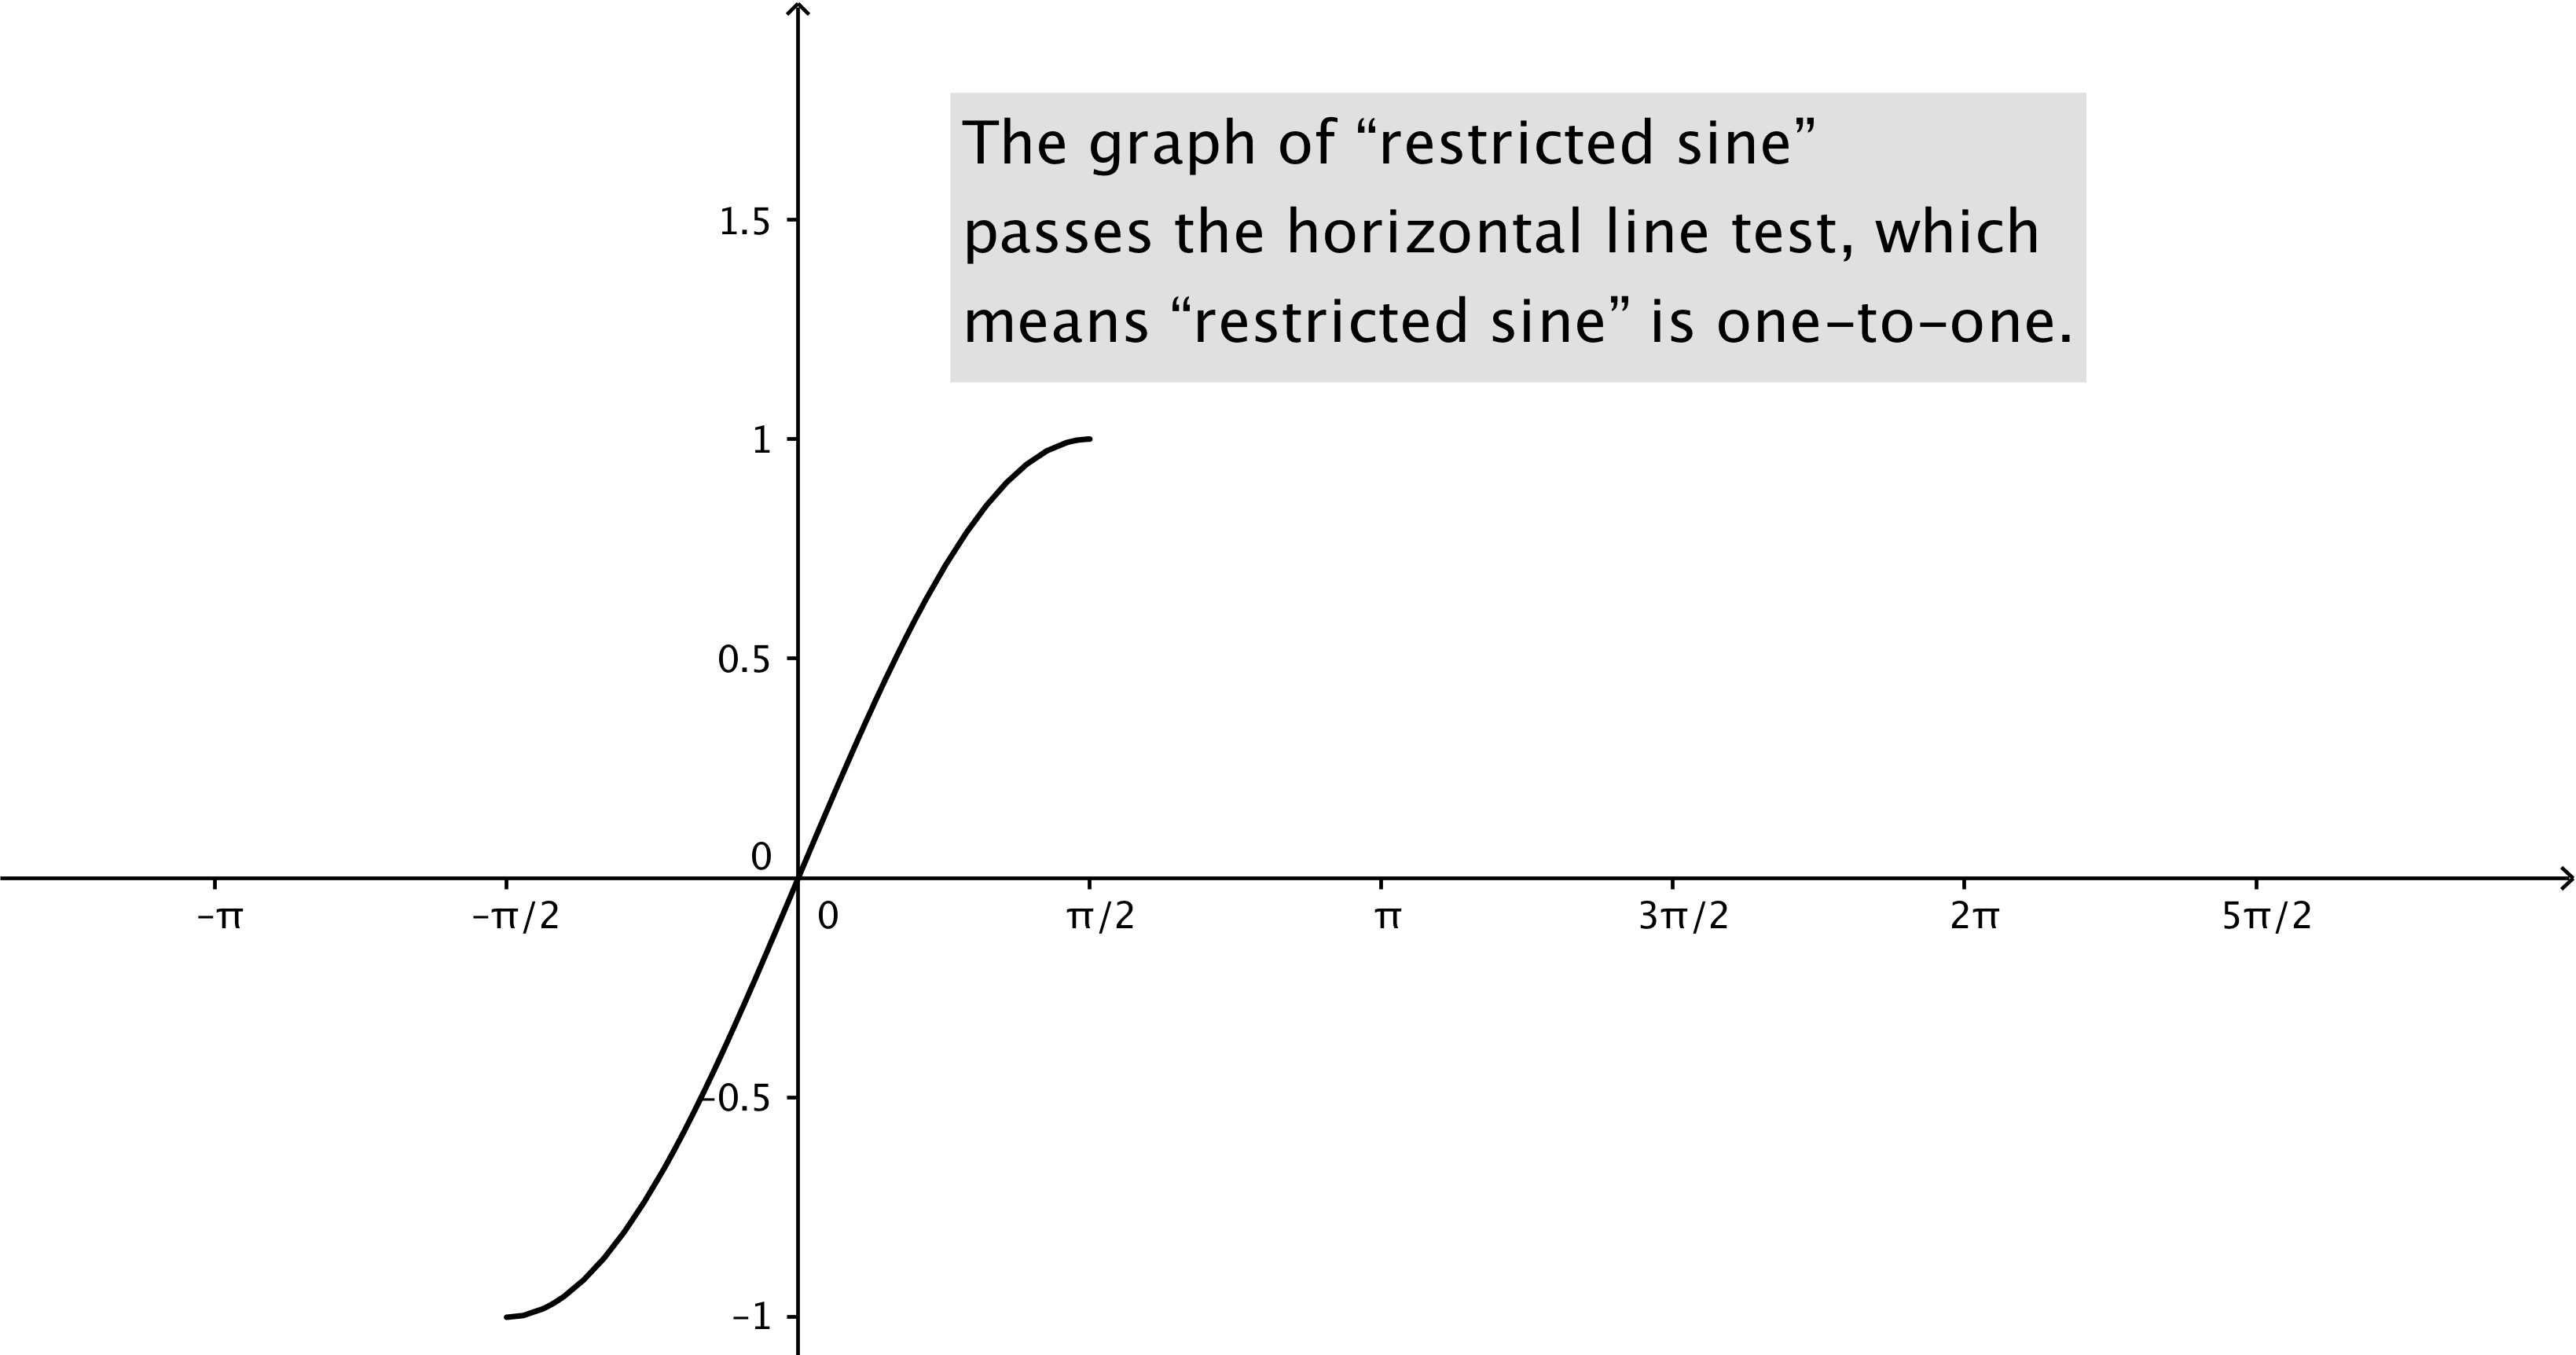
\includegraphics[scale = 0.4]{figure4.png}
    \end{image}
    So, the range of $\sin^{-1}$ is $[-\pi/2, \pi/2]$.
    Since $\pi$ is not in this range, $\pi$, is \emph{never} a possible output of $\sin^{-1}$.
  \end{freeResponse}
\end{problem}

%problem4
    \begin{problem}
  Simplify each of the following expressions.
  \begin{enumerate}
    \item
      $\cos^{-1} \bigl( \sin(\pi/2) \bigr)$
      \begin{freeResponse}
        By the unit circle, $\sin(\pi/2) = 1$, and so we are looking for $\cos^{-1}(1)$.
        The range of $\cos^{-1}$ is $[0, \pi]$, and so, by properties of inverse functions, $\cos^{-1}(1) = 0$.
      \end{freeResponse}

    \item
      $\tan \bigl( \sin^{-1}(4/x ) \bigr)$
      \begin{freeResponse}
        Let $\theta = \sin^{-1}(4/x)$, then $\sin(\theta) = 4/x$.
        We can then draw the corresponding right triangle:
        \begin{image}
          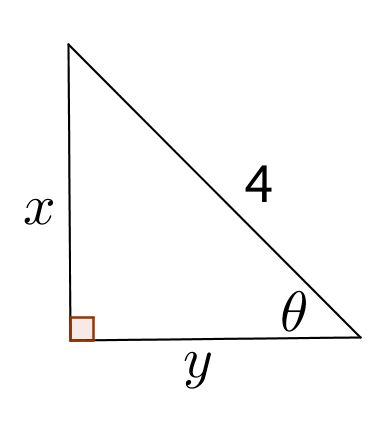
\includegraphics[scale = 0.8]{figure5.png}
        \end{image}
        Calling the adjacent side $y$, by the Pythagorean Theorem we obtain
        \begin{align*}
          x^2 = 16 + y^2 &\implies y = \pm\sqrt{x^2 - 16}, \\
                         &\implies y = \sqrt{x^2 - 16}.\\
                         &\hspace{-0.5em} \mbox{\parbox[b][]{6cm}{(since we assume the side of a triangle can't have negative length)}}
        \end{align*}
        Then
        \begin{align*}
          \tan \left( \sin^{-1} \left(4/x \right) \right) &= \tan( \theta), \\
                                                                   &= \frac{4}{y}, \\
                                                                 &= \frac{4}{\sqrt{x^2 - 16}}.
        \end{align*}
      \end{freeResponse}
  \end{enumerate}
\end{problem}  

%problem5
\begin{problem}
  A table of values for $f$ and $f'$ is shown below.
  Suppose that $f$ is a one-to-one function and $f^{-1}$ is its inverse.
  \begin{center}
    \begin{tabular}{ccc}
\hline
      $x$ & $f(x)$ & $f'(x)$\\
\hline \hline
      1 & 3 & 4\\

      3 & 4 & 5\\

      4 & 6 & 3\\
\hline
    \end{tabular}
  \end{center}

  \begin{enumerate}
    \item Evaluate $f^{-1}(f(x))$ at $x = 3$.
      \begin{freeResponse}
         $ f^{-1}(f(3)) = f^{-1}(4) = 3$
      \end{freeResponse}


    \item Evaluate $\ddx f(f(x))$ at $x = 3$.
      \begin{freeResponse}

        \begin{align*}
          \ddx f(f(x)) = f'(f(x)) \cdot f'(x) &\implies \eval{\ddx}_{x = 3} f(f(x)) = f'(f(3)) \cdot f'(3)\\
          &= f'(4) \cdot 5 = 3 \cdot 5 = 15
        \end{align*}
      \end{freeResponse}


    \item Evaluate $\ddx\ln((f(x))$ at $x = 3$.
      \begin{freeResponse}

        \begin{align*}
          \ddx\ln((f(x)) = \frac{f'(x)}{f(x)} \\
          &\implies \eval{\ddx \ln(f(x))}_{x = 3} = \frac{f'(3)}{f(3)} = \frac{5}{4}
        \end{align*}
      \end{freeResponse}


    \item Evaluate $f^{-1}(x)$ at $x = 3$.
      \begin{freeResponse}
	$ f^{-1}(3) = 1 \iff 3 = f(1)$
      \end{freeResponse}


    \item Evaluate $\ddx f^{-1}(x)$ at $x = 3$.
      \begin{freeResponse}
        \begin{align*}
          \ddx f^{-1}(x) &= \frac{1}{f'(f^{-1}(x))} \\
          &\implies \eval{\ddx f^{-1}(x)}_{x = 3} = \frac{1}{f'(f^{-1}(3))} \\
          &= \frac{1}{f'(1)} = \frac{1}{4}
        \end{align*}
      \end{freeResponse}
      
      \item Evaluate $\lim_{x \to 4} \frac{f(x)-f(4)}{x-4}$
      \begin{freeResponse}
$\lim_{x \to 4} \frac{f(x)-f(4)}{x-4} = f'(4)=3$
      \end{freeResponse}
  \end{enumerate}
\end{problem}


%problem6
\begin{problem}
Find the derivative of $f^{-1}$ at the following points without solving for $f^{-1}$.
	\begin{enumerate}
	
	\item  $f(x) = x^2 + 1$ (for $x \geq 0$) at the point $(5,2)$.  
		\begin{freeResponse}
		$(f^{-1})'(5) = \frac{1}{f'(2)}$.  Since $f'(x) = 2x$, $f'(2) = 4$.  Thus, $(f^{-1})'(5) = \frac{1}{4}$.  
		\end{freeResponse}

	\item  $f(x) = x^2 - 2x - 3$ (for $x \leq 1$) at the point $(12, -3)$.  
		\begin{freeResponse}
		$(f^{-1})'(12) = \frac{1}{f'(-3)}$.  Since $f'(x) = 2x - 2$, $f'(-3) = -6 - 2 = -8$.  Thus, $(f^{-1})'(12) = - \frac{1}{8}$. 
		\end{freeResponse}
	\end{enumerate}
\end{problem}


%problem7
\begin{problem}

  Find the slope of the tangent line to the curve $y = f^{-1}(x)$ at $(4,7)$ if the slope of the tangent line to the curve $y=f(x)$ at $(7,4)$ is $\frac{2}{3}$.
  \begin{freeResponse}
    Note that the statement ``the slope of the tangent line to the curve $y=f(x)$ at $(7,4)$ is $\frac{2}{3}$" specifically means that $f'(7) = \frac{2}{3}$.
    The slope of the tangent line to the curve $y = f^{-1}(x)$ at $(4,7)$ is $(f^{-1})'(4)$, and so we use the formula for the derivative of the inverse function to compute: $(f^{-1})'(4) = \frac{1}{f'(7)} = \frac{1}{\frac{2}{3}} = \frac{3}{2}$.
  \end{freeResponse}
\end{problem}

%problem8
\begin{problem}
Find the derivatives of the following functions:
	\begin{enumerate}
	
	%part a
	\item  $f(x) = \sec^{-1} (\sqrt{x})$.
		\begin{freeResponse}
		$f'(x) = \frac{1}{\sqrt{x} \sqrt{x - 1}} \cdot \frac{1}{2} x^{-\frac{1}{2}} = \frac{1}{2x\sqrt{x-1}}$
		\end{freeResponse}
		
		
		
	%part b
	\item  $g(x) = \ln (\sin^{-1}(x))$.
		\begin{freeResponse}
		$g'(x) = \frac{1}{\sin^{-1}(x)} \cdot \frac{1}{\sqrt{1-x^2}}$.
		\end{freeResponse}
		
		
		
	%part c
	\item  $h(x) = \frac{1}{\tan^{-1}(x^2 + 4)}$.  
		\begin{freeResponse}
		$h'(x) = - \left( \tan^{-1}(x^2 + 4) \right)^{-2} \cdot \frac{1}{1 + (x^2 + 4)^2} \cdot (2x)$.
		\end{freeResponse}
		
		
		
	\end{enumerate}
		
		
\end{problem}


%problem9
\begin{problem}
A boat sails directly toward a 100-meter skyscraper that stands on the edge of a harbor.  The angular size $\theta$of the building is the angle formed by lines from the top and bottom of the building to the observer (see figure below).
    \begin{image}
      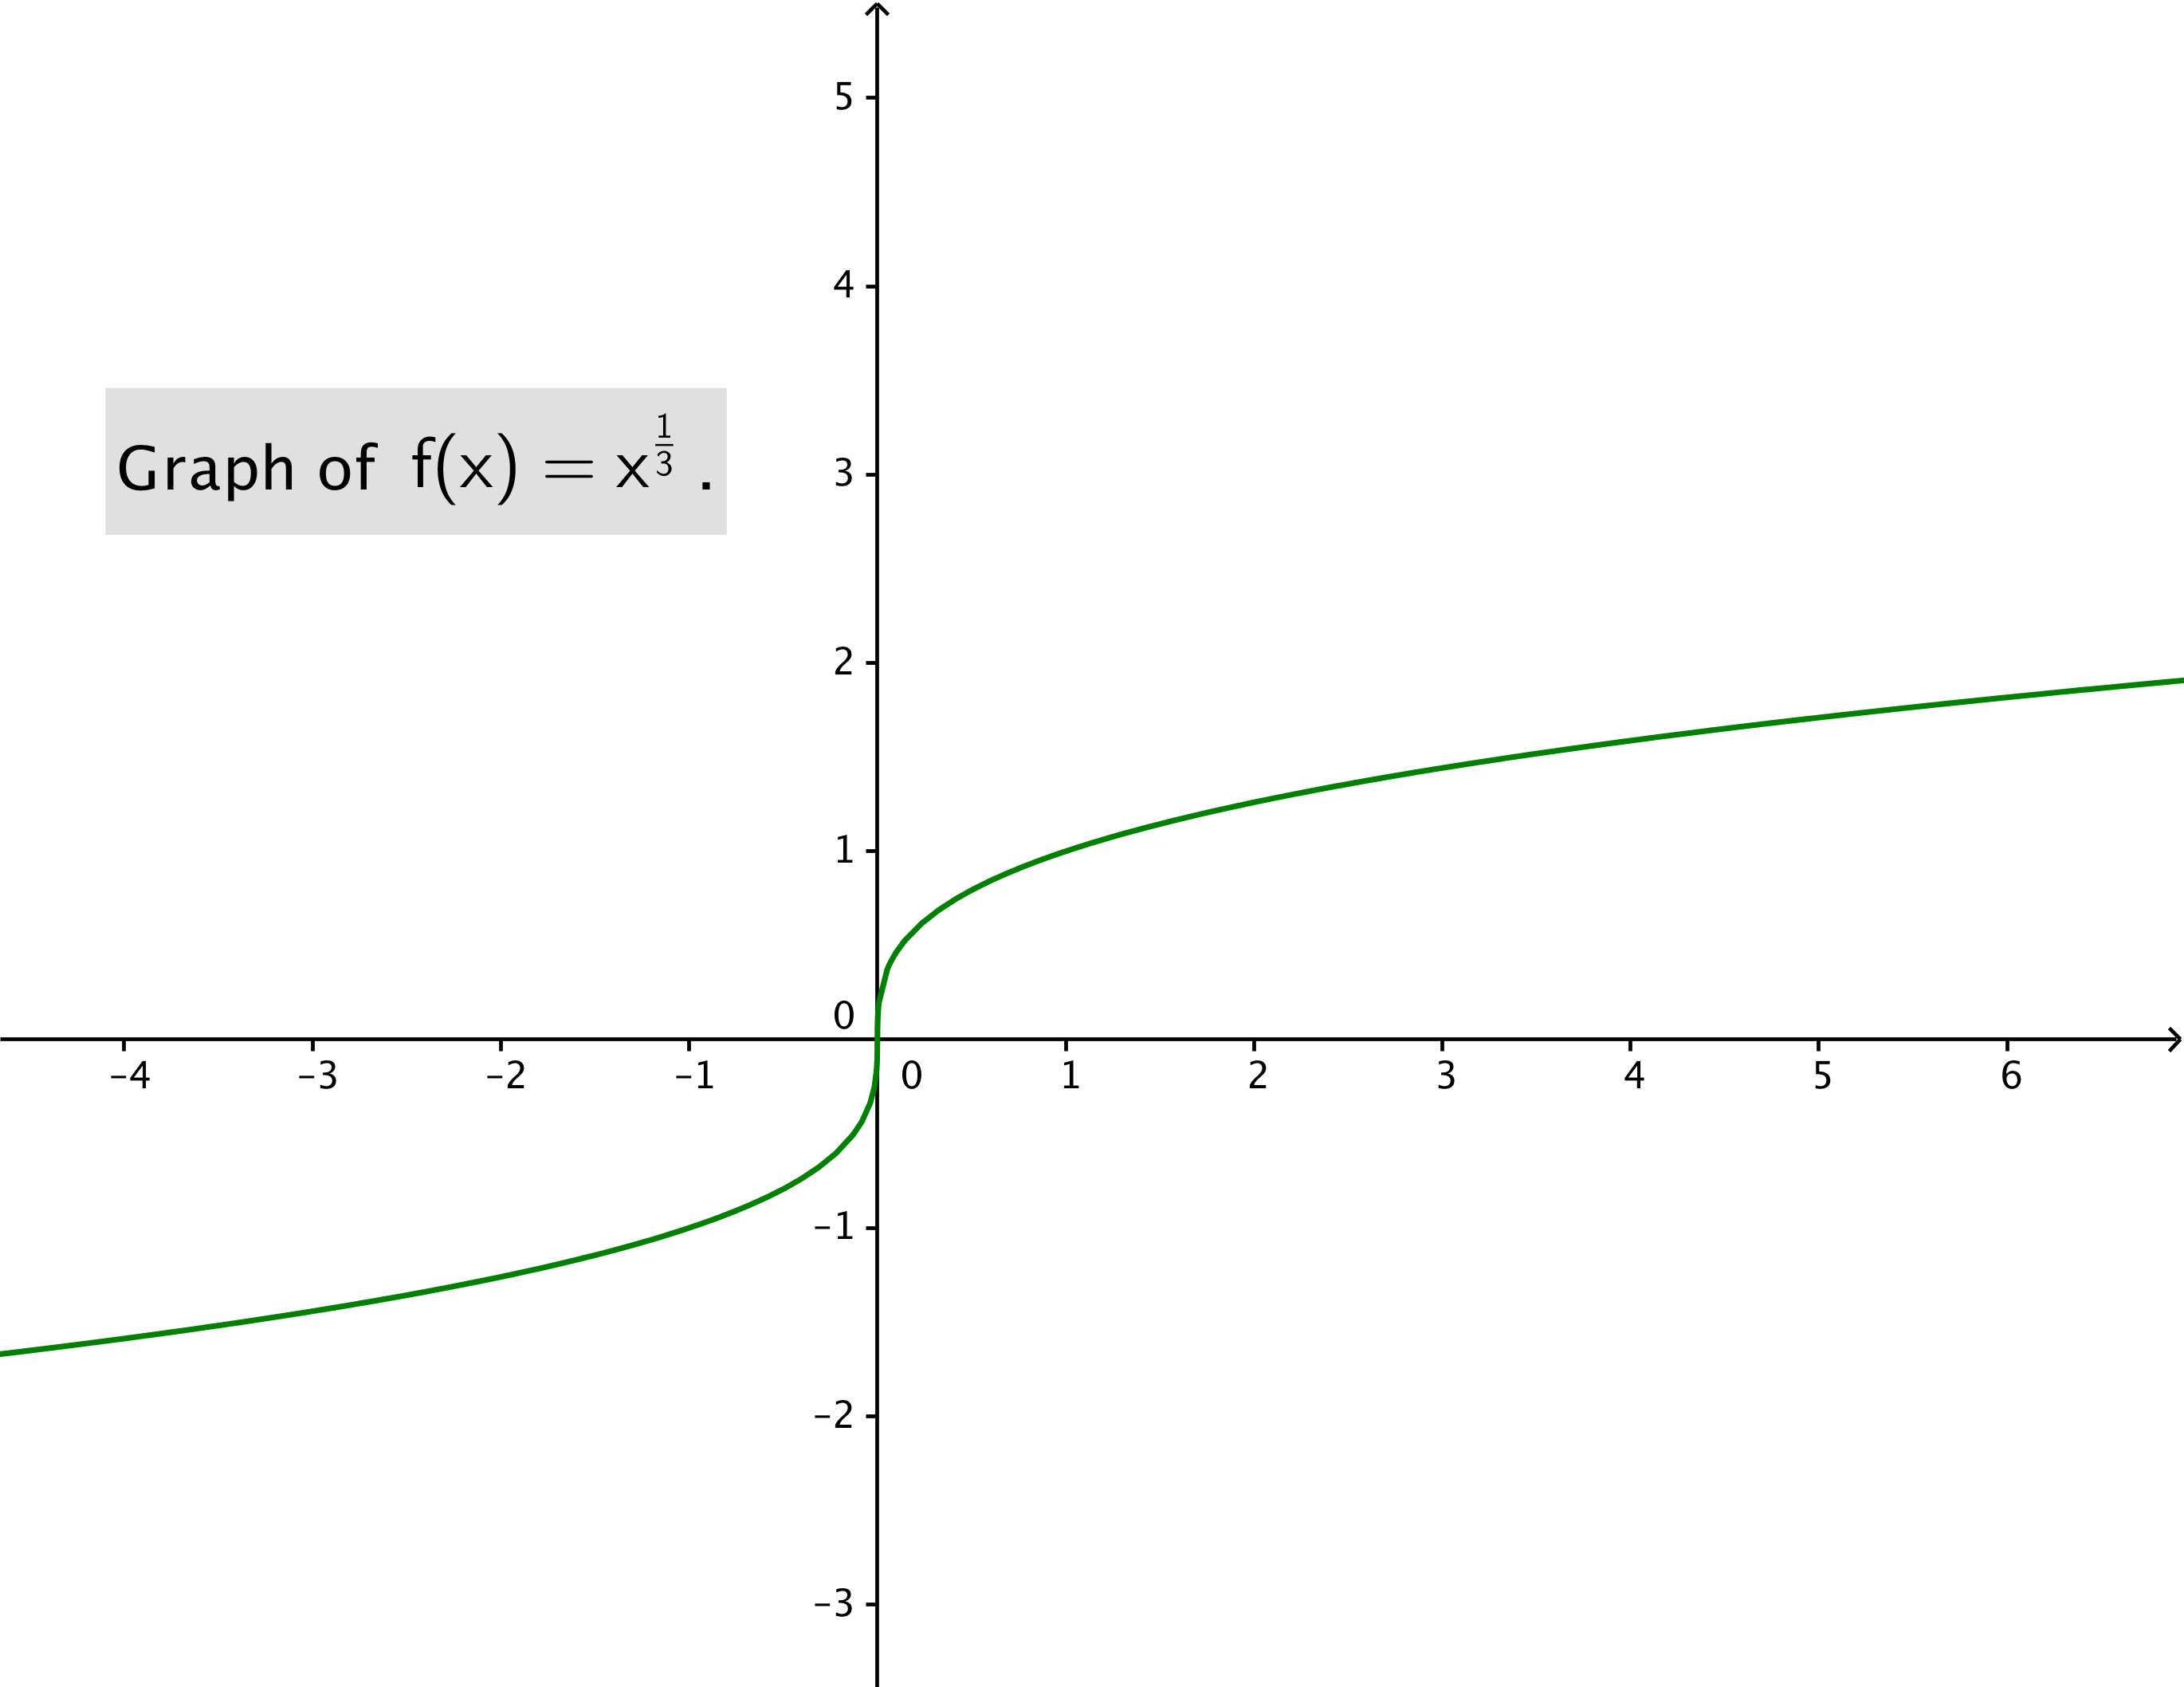
\includegraphics[scale = 0.7]{figure6.png}
    \end{image}

\begin{enumerate}
	\item Express the angle $\theta$ as the function of $x$, the distance of the boat from the building.
	\begin{freeResponse}
	\begin{align*}
	\tan\theta&=\frac{100}{x}\\
	\theta&=\tan^{-1}\left( \frac{100}{x} \right)
	\end{align*}
	\end{freeResponse}
	
	\item The boat is sailing directly toward the skyscraper at $3$ m/s.  Find $\dd[\theta]{t}$ when the boat is $x=300$m from the building.
	\begin{freeResponse}
	\begin{align*}
	\frac{d\theta}{dt}&=\dd{t}\tan^{-1}\left( \frac{100}{x} \right)\\
	&=\dd{x}\tan^{-1}\left( \frac{100}{x} \right)\dd[x]{t}\\
	&=\frac{1}{1+\frac{100}{x}^2} \cdot \frac{-100}{x^2} \dd[x]{t}\\
	&=\frac{1}{1+\frac{100}{x}^2} \cdot \frac{-100}{x^2} \cdot (-3)\\
	&=\frac{300}{x^2+100^2}\\\\
	\eval{\dd[\theta]{t}}_{x=300}&=\frac{300}{300^2+100^2}\\
	&=\frac{3}{900+100}\\
	&=\frac{3}{1000}\\
	&=0.003\ \text{rad/sec}
		\end{align*}
		Alternatively, this problem could be done without inverse trigonometry.\\
	\begin{align*}
	\tan\theta&=\frac{100}{x}\\
	\dd{t}(\tan\theta)&=\dd{t} \left(\frac{100}{x}\right)\\
	\sec^2\theta \dd[\theta]{t}&=\frac{-100}{x}\dd[x]{t}
	\end{align*}
	
	We have to evaluate $\sec^2\theta$ at the moment when $x=300$m\\
	    \begin{image}
      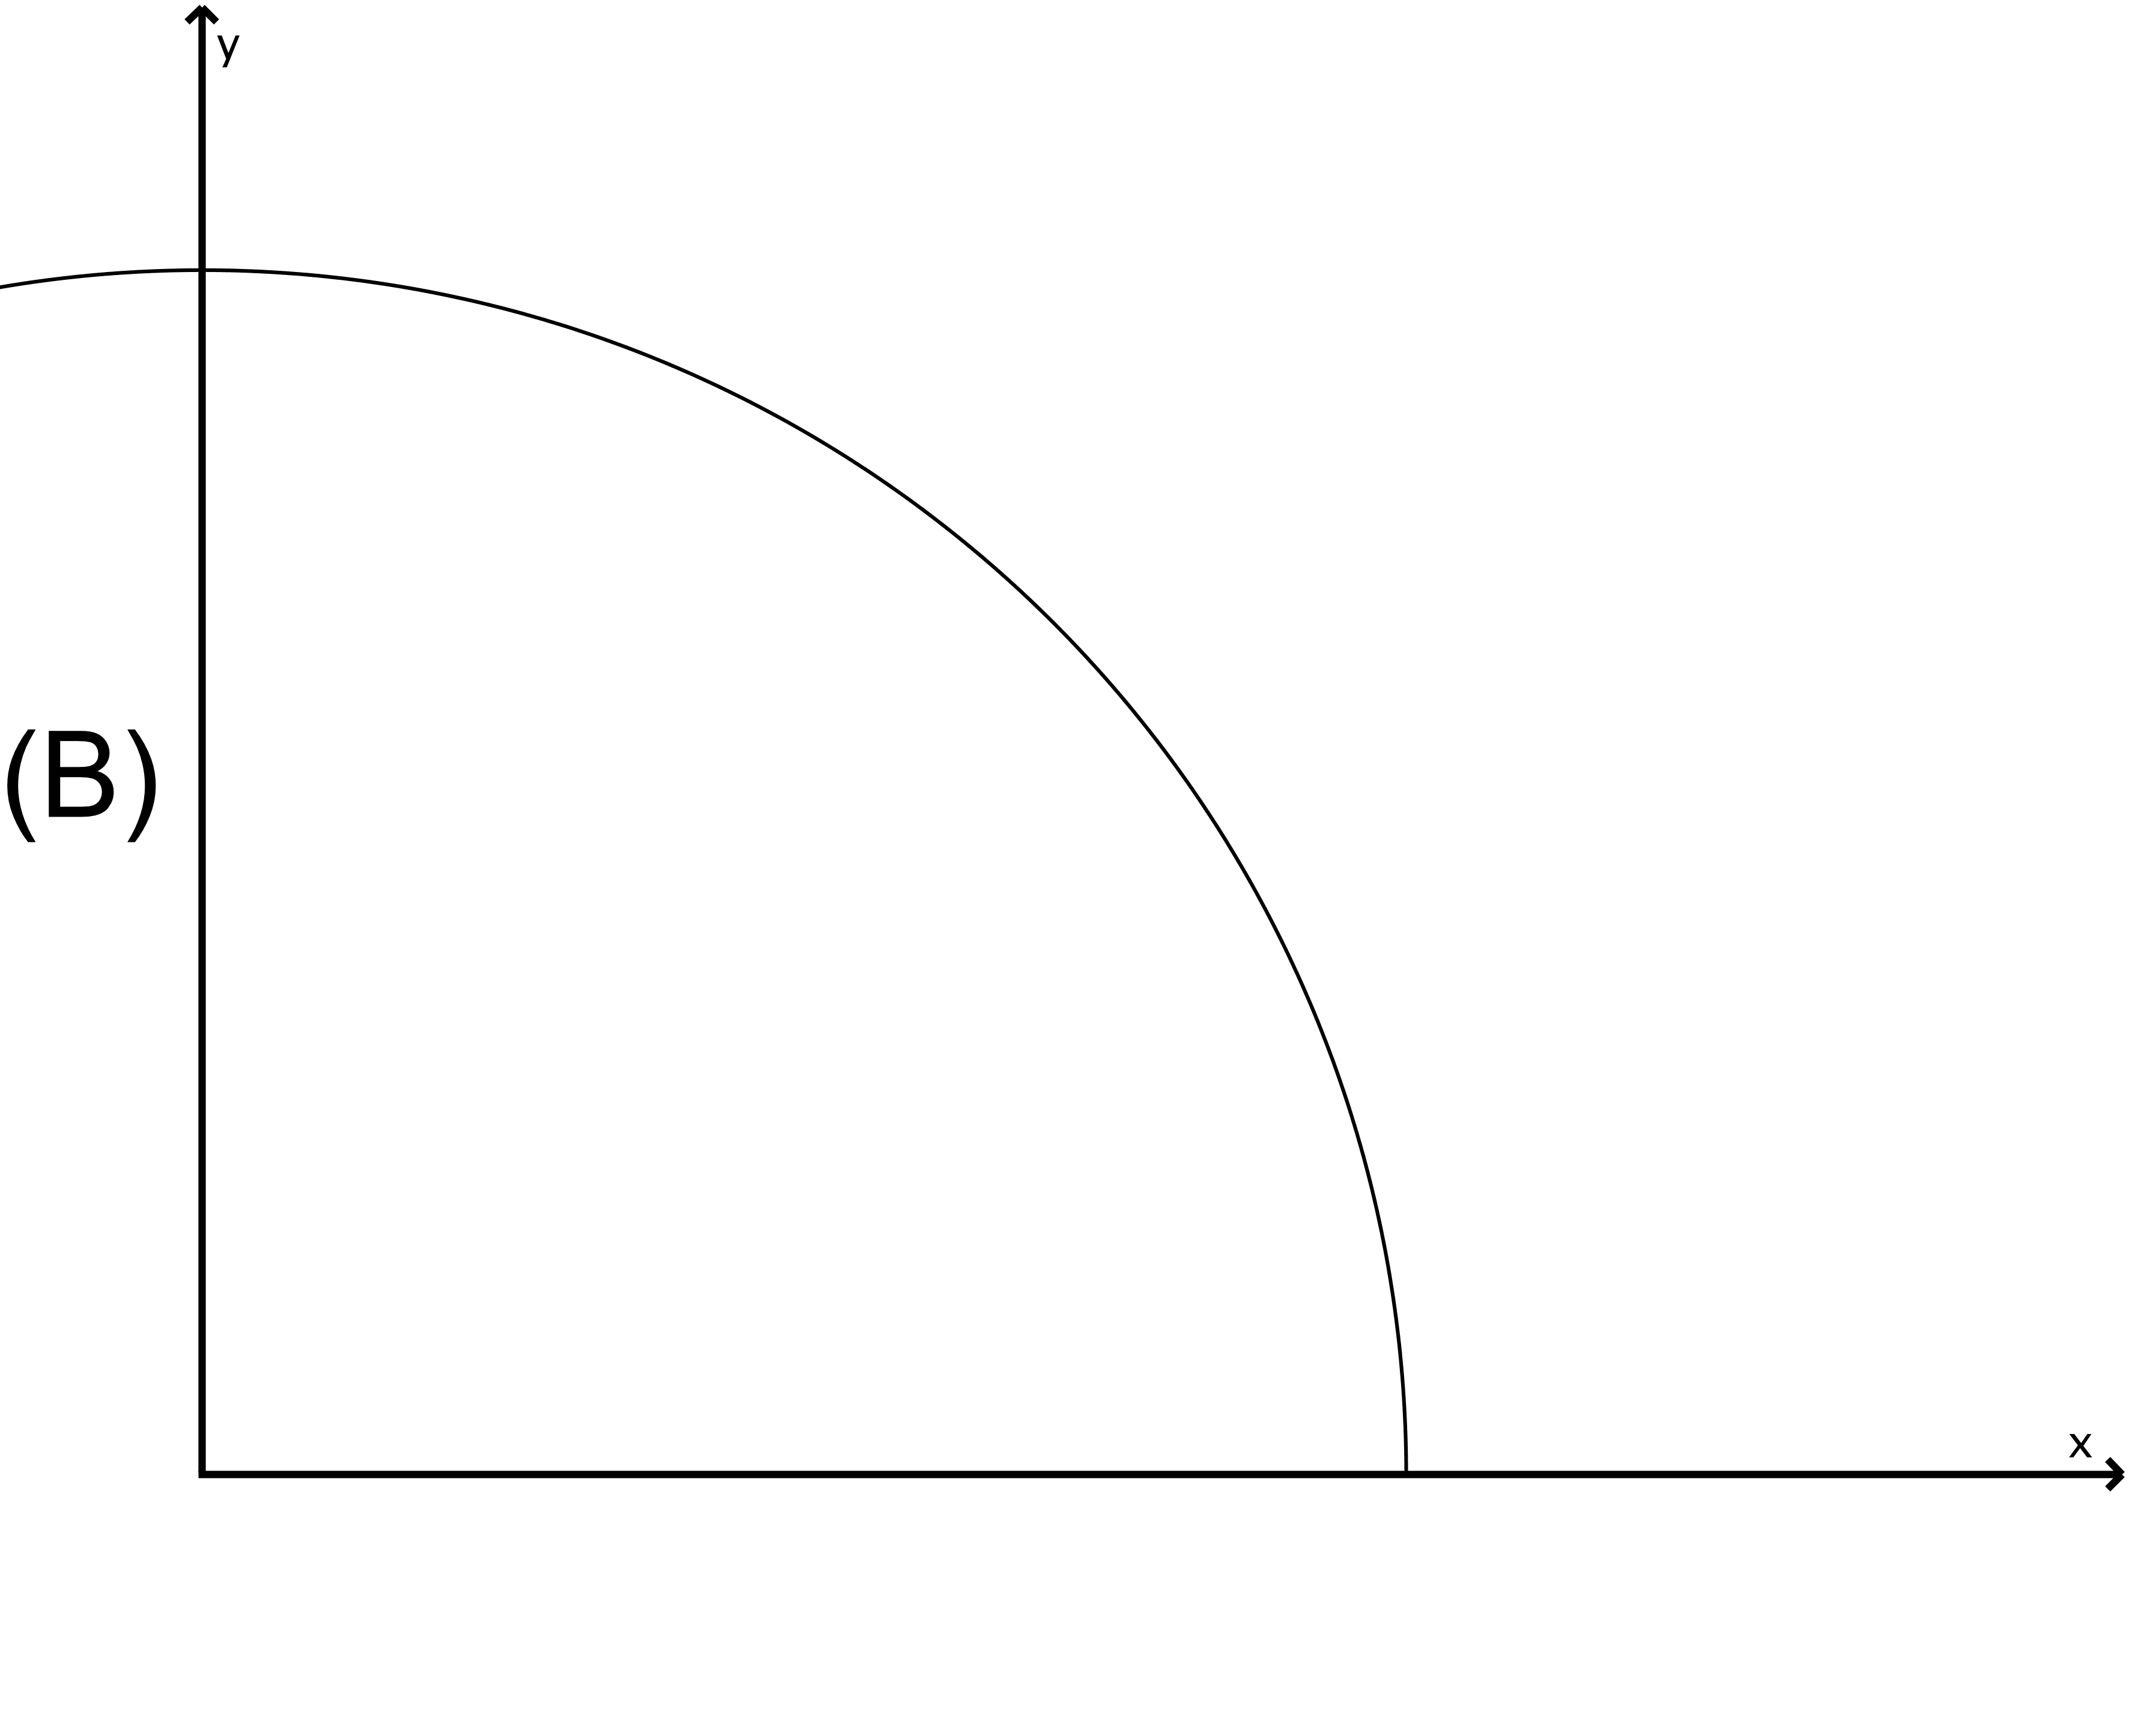
\includegraphics[scale = 0.7]{figure7.png}
    \end{image}
	Using the triangle above, we have:\\\\
	$\sec\theta=\frac{\sqrt{300^2+100^2}}{300}=100\frac{\sqrt{3^2+1^2}}{300}=\frac{\sqrt{10}}{3}$, we obtain:\\
	\begin{align*}
	\left(\frac{\sqrt{10}}{3}\right)^2 \eval{\dd[\theta]{t}}_{x=300}&=-\frac{100}{300^2}(-3)\\
	\eval{\dd[\theta]{t}}_{x=300}&=\frac{1}{100} \cdot\frac{9}{10}=\frac{3}{1000}\  \text{rad/sec}
	\end{align*}

	\end{freeResponse}
\end{enumerate}
\end{problem}

\end{document} 


















